\section{Introduction}
	\subsection{Digital Radio Frequency Memory}
	\noindent Digital Radio Frequency Memory (DRFM) systems digitize and store incoming RF input signals at specific frequencies and bandwidths. The captured signals undergo time delays, frequency shifts and amplitude scalings, after which they are retransmitted. DRFM is used in order to synthesize false targets for radar systems by exploiting the radar assumptions of target identification. This is achieved by retransmitting a time delayed, amplitude scaled and frequency shifted coherent replica of the inputted signal, thereby making it, from the radar's perspective, indistinguishable from other genuine signals\cite{SJROOME}.\\ \newline The reason why a radar system is deceived is due to its fundamental operation. For example, a pulsed radar operates by transmitting pulses on a target and measuring the time delay and frequency shift of the return pulse from the target in order to infer information about a target's location and velocity. The implications of this are such that if we simulate echos with certain frequency shifts and time delays it is possible for a radar to identify a target incorrectly.\\ \newline An illustration of a DRFM system may be seen in Fig.~\ref{fig:DRFM_Intro}. It can be seen that the input signal is mixed down to intermediate frequency and then is sampled by an Analog to Digital Converter (ADC). The sample rate of the ADC is equal to the bandwidth of the incoming RF signal as the ADC is sampling complex I/Q data. The digitized signal is then stored in memory and may be manipulated by means of the control interface. The control interface is used to designate the various time delays, frequency shifts and amplitude scalings. 
	\subsection{FPGA based Architecture}
	\noindent Due to the high data rates and the Digital Signal Processing (DSP) requirements the implementation of DRFM systems are highly suitable to Field Programmable Gate Arrays (FPGA). Therefore this paper describes the design and implementation of a DRFM system on a low cost FPGA, namely the Altera MAX 10 \cite{DE10lite}. 
	\begin{figure}[h!]
		\centering
		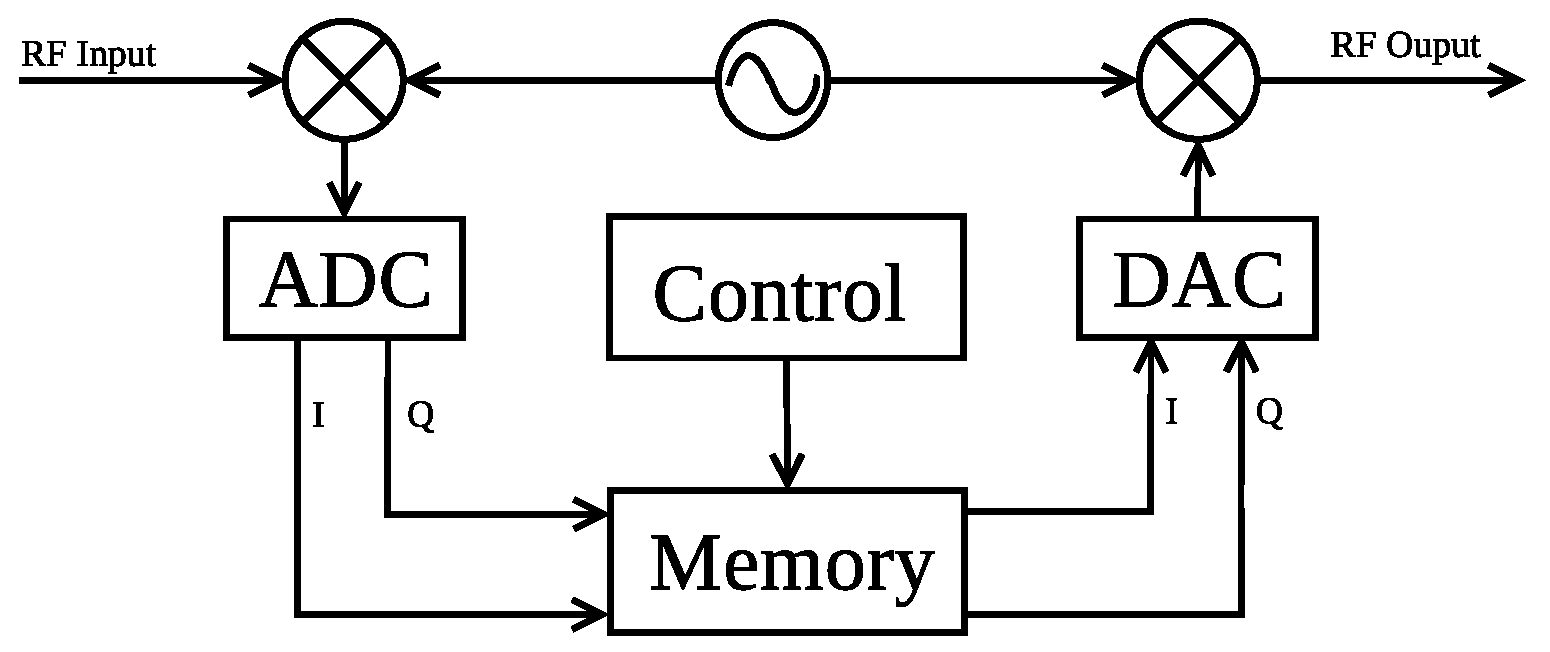
\includegraphics[width=0.8\linewidth]{img/DRFM_Intro}
		\caption{Illustration of DRFM System}
		\label{fig:DRFM_Intro}
	\end{figure}
	\subsection{Plan of Development}
	\noindent This paper begins by discussing the conceptual design of the proposed DRFM architecture by giving an overview of its implementation. After which, the details of each subsystem is described. Finally, results are shown and conclusions are drawn based on the prototype design.

		


